\section{\emph{Smart Assistive Posture Device}}
\label{sec:posturedevice}

\begin{figure}[ht]
  \centering
  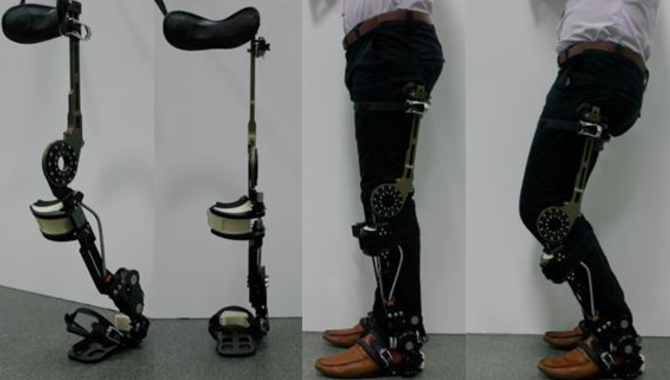
\includegraphics[scale=0.3]{gambar/contoh-posture-device.png}
  \caption{\emph{Smart assistive posture device} dengan \emph{human-chair system} \citep{cit:choi2015}.}
  \label{fig:contohposturedevice}
\end{figure}

\emph{Smart assistive posture device} merupakan sebuah perangkat cerdas yang umumnya digunakan di industri untuk membantu pekerja dalam meringankan ketegangan otot.
Berbagai perangkat dengan fungsi tersebut telah banyak dikembangkan,
  salah satunya adalah perangkat dengan \emph{human-chair system} \citep{cit:choi2015}.
Perangkat dengan sistem tersebut memiliki fungsi untuk mengurangi ketegangan pada otot kaki bagi pengguna ketika posisi duduk.
Pada perangkat tersebut,
  pengguna dimodelkan sebagai empat batang saling terhubung yang terdiri atas bagian atas tubuh, paha, betis, dan telapak kaki.
Seperti pada gambar \ref{fig:contohposturedevice},
  Perangkat dengan sistem tersebut sendiri merepresentasikan dua batang pada paha dan betis untuk membantu menyangga pengguna di kedua bagian tersebut.
